\subsection{Level2.2: $z=x^2 + y^2$ について}
\subsubsection{プログラムソース(変更部分)}
以下の図\ref{cp22}に変更部分のみを示す。
	\begin{figure}[H]
        \caption{Level2.2 変更点}
		\label{cp22}
		\fontsize{10pt}{10pt}\selectfont
      	\begin{shadebox}
        	\begin{verbatim}
			//main 関数直後
			f( argc != 3 ){
			(略)
			}else{
			(略)
			alpha = atof(argv[2]); 
			(略)
			}
			
			//f 関数内
			//  z = x;
			  z = x*x + y*y;

			//pd_x 関数内
			//  z_dx = 1;
			  z_dx = 2*x;

			//pd_y 関数内
			//  z_dy = 0;
			  z_dy = 2*y;
        	\end{verbatim}
      	\end{shadebox}
     \end{figure}

\subsubsection{観察意図と観察方法}
seed値を固定してalpha 値を変動させることで,探索点の刻み幅による探索の最適性及び
効率性を検討する。
alpha 値を変更することで探索幅も変動することから,以下の2つのような予想が立てられる。
1, alpha 値が大きければ探索点の刻み幅も大きくなり,効率性を向上できるが,最適性が低下
する。
2, alpha 値が小さければ探索点の刻み幅が小さくなるため,最適性を向上できるが,効率性
が低下する。\\
効率性の観察方法は,seed値を固定しalpha 値を変動させた際のstep 数の推移を
各seed 値(範囲1000-10000 1000刻み)ごとに表して行う。
効率性の検討はグラフより,各seed 数で最小step 数のalpha 値を読み取り,
最も優れたalpha 値を多数決で決定し,それをこのプログラムの最大効率であると決定,
改善点を考察する。\\
また,srand 関数にコマンドライン引数のseed 値が渡されているため,
rand 値は同じseed 値 を入力している限り,一定である。よって,同一seed 値 において,
乱数を考慮しての複数実行,実行結果の平均値取得等はしない。\\
最適性の観察方法は,seed値を固定しalpha 値を変動させた際の終了時座標,これと
傾きが0になっている座標(ここでは0,0)との差の推移を各seed 値
(範囲1000-10000 1000刻み)ごとにグラフで表す。
最適性の検討はグラフからその差が最小のalpha の値を各seedから読み,最も優れた
alpha 値を多数決で決定する。
そのalpha 値をこのプログラムの最大最適値 であると決定し,改善点を考察する。

\subsubsection{実行結果}
  \begin{enumerate}
  \renewcommand{\labelenumi}{\arabic{enumi}}

  \item 効率性について\\
	効率性の観察のための手法として,各seed値(1000-10000の1000刻み10種),
	各alpha値(0.001 と 0.1-1.0(0.1刻み)の計11種) ごとに
	最終step数をplot していき,その推移傾向を観察することで行った。\\
	以下の図\ref{stepgraph1}がその結果である。

  \begin{figure}[H]
	\begin{center} %センタリングする
	  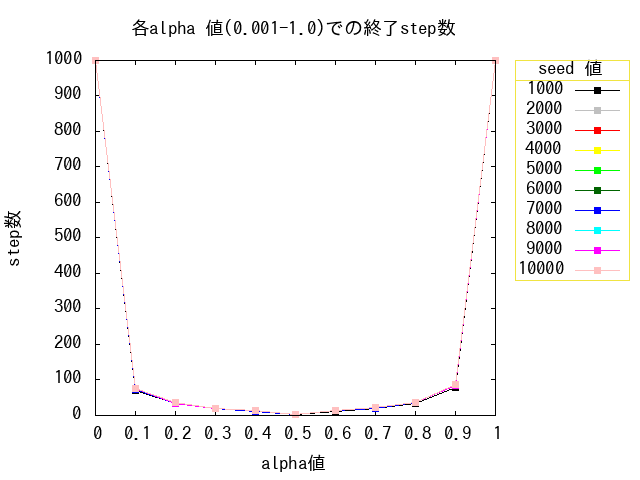
\includegraphics[width=9cm]{../steepestsearch2-2/createStepGraph/StepGraph.png}
	  \caption{各alpha値(0.001-1.0) での終了step数} %タイトルをつける
	  \label{stepgraph1} %ラベルをつけ図の参照を可能にする
	\end{center}
  \end{figure}

  alpha 値が 0.001, 1.0 の時に step数が1000となり,alpha 値 0.1-0.9 までの
  点の差が見えづらい。よって,alpha 値が0.1-0.9 の範囲の最終step数のグラフも
  図\ref{stepgraph2}に用意した。
  \begin{figure}[H]
	\begin{center} %センタリングする
	  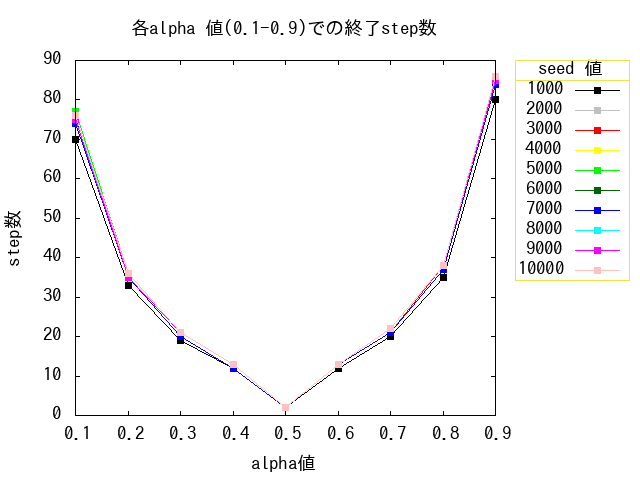
\includegraphics[width=9cm]{../steepestsearch2-2/createStepGraph/StepGraph2.png}
	  \caption{各alpha値(0.1-0.9) での終了step数} %タイトルをつける
	  \label{stepgraph2} %ラベルをつけ図の参照を可能にする
	\end{center}
  \end{figure}


  \item 最適性について\\
	最適性の観察のための手法として,各seed値(1000-10000の1000刻み10種),
	各alpha値(0.001 と 0.1-1.0(0.1刻み)の計11種) ごとに
	終了座標の誤差(x,yの合計)をplot していき,その推移傾向を観察することで行った。\\
	以下の図\ref{diffgraph1}がその結果である。


  \begin{figure}[H]
	\begin{center} %センタリングする
	  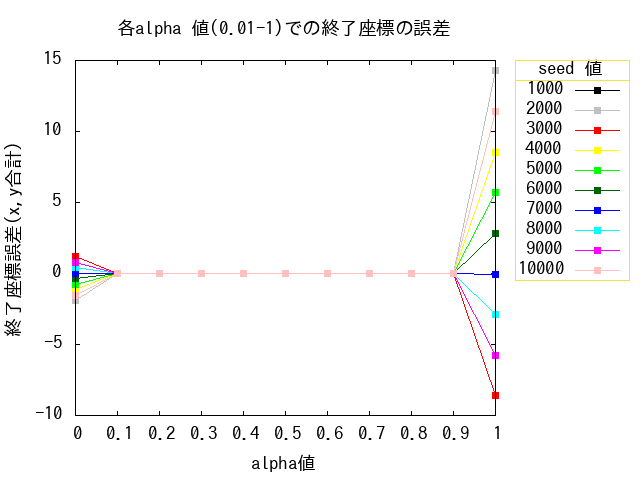
\includegraphics[width=9cm]{../steepestsearch2-2/createDiffGraph/DiffGraph.png}
	  \caption{各alpha値(0.001-1.0) での終了座標誤差(x,y合計)} %タイトルをつける
	  \label{diffgraph1} %ラベルをつけ図の参照を可能にする
	\end{center}
  \end{figure}

  alpha 値が 0.001, 1.0 の時に 最大合計誤差10を超え,alpha 値 0.1-0.9 までの
  点の差が見えづらい。よって,alpha 値が0.1-0.9 の範囲の合計誤差のグラフも
  図\ref{stepgraph2}に用意した。
  \begin{figure}[H]
	\begin{center} %センタリングする
	  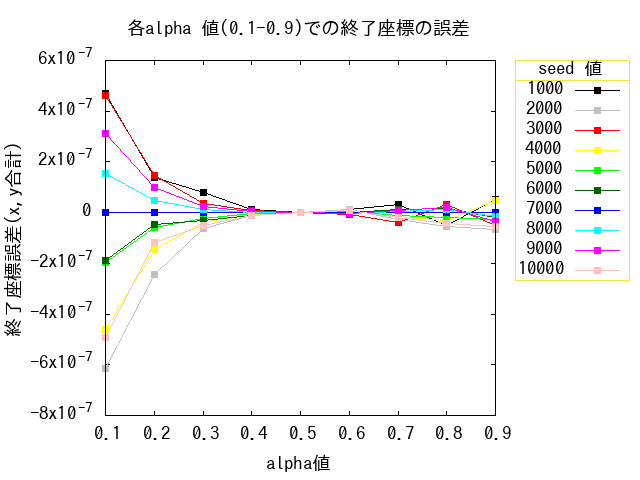
\includegraphics[width=9cm]{../steepestsearch2-2/createDiffGraph/DiffGraph2.png}
	  \caption{各alpha値(0.1-0.9) での終了座標誤差(x,y合計)} %タイトルをつける
	  \label{diffgraph2} %ラベルをつけ図の参照を可能にする
	\end{center}
  \end{figure}

  \end{enumerate}

\subsubsection{考察}
まず,効率性についての考察を行う。\\
図\ref{stepgraph1}より,最終step数が1000回以内に収まるのが,$0.001 < alpha < 1.0$
の範囲であることがわかる。このことから,alpha 値が小さすぎると探索できる
範囲が狭まり,最適解まで届かなかったと推察する。 図\ref{stepgraph2}からは,
総step数が1番低い点のalpha 値が 0.5 であり,0.5 から離れるごとにstep 数が
増加する傾向にあることがわかる。alpha値が0.5 の時に総step数が最小となった理由を,
プログラム内の探索点移動に用いられている式より考察する。\\
$x = x - alpha*pd_x(x,y);$\\
この式のpd\_x(x,y) はxについての偏微分であるため,置き換えると\\
$x = x - alpha*2x;$\\
となる。この式に alpha = 0.5 を代入すると x には '0' が入ることとなるため,
移動後のx座標がちょうど傾きが0になる点(最終的に移動したい最適解)になる。
yについても同様にしてalpha = 0.5 の時に1回移動後の座標は'0'となる。\\
このことから, alpha = 0.5 という値は 今回探索した $x^2 + y^2$ の式において
あらゆる座標から最適解の座標を求めることができる値であることがわかる。\\

次に,最適性について\\
効率性の考察にて
図\ref{stepgraph1}より,最終step数が1000回となるのが$alpha=0.001 , alpha=1.0$
で,言い換えると$alpha=0.001 , alpha=1.0$のとき最適解との誤差が大きい。\\
このことが,終了座標誤差を表す図\ref{diffgraph1}からも読み取れる。
図\ref{diffgraph2}からは効率性と同じく alpha=0.5 に最適性が最も高いことがわかる。
さらにalpha=0.5 の点へのグラフの収束の度合いにも alpha が0.5より小さい時と
大きい時で差がある。これは,alphaが0.5より小さい場合の最適解からの誤差は探索点が
単純に最適解に届かなかったものであるが,alpha が0.5より大きい場合では
最適解付近まで探索点が到達したが探索点の移動幅の大きさが影響し最適解には
至らなかったというもの,という差によるものと推察する。

